%%%%%%%%%%%%%%%%%%%%%%%%%%%%%%%%%%%%%%%%%%%%%%%%%%%%%%%%%%%%%%%%%%%%%%%%%%%%%%%%
%2345678901234567890123456789012345678901234567890123456789012345678901234567890
%        1         2         3         4         5         6         7         8

\documentclass[letterpaper, 10 pt, conference]{ieeeconf}
% Comment this line out if you need a4paper

%\documentclass[a4paper, 10pt, conference]{ieeeconf}
% Use this line for a4 paper

\IEEEoverridecommandlockouts
% This command is only needed if
% you want to use the \thanks command

\overrideIEEEmargins
% Needed to meet printer requirements.

%In case you encounter the following error:
%Error 1010 The PDF file may be corrupt (unable to open PDF file) OR
%Error 1000 An error occurred while parsing a contents stream. Unable to analyze the PDF file.
%This is a known problem with pdfLaTeX conversion filter. The file cannot be opened with acrobat reader
%Please use one of the alternatives below to circumvent this error by uncommenting one or the other
%\pdfobjcompresslevel=0
%\pdfminorversion=4

% See the \addtolength command later in the file to balance the column lengths
% on the last page of the document

% The following packages can be found on http:\\www.ctan.org
\usepackage{graphics} % for pdf, bitmapped graphics files
\usepackage{epsfig} % for postscript graphics files
\usepackage{mathptmx} % assumes new font selection scheme installed
\usepackage{times} % assumes new font selection scheme installed
\usepackage{amsmath} % assumes amsmath package installed
\usepackage{amssymb}  % assumes amsmath package installed
\usepackage{verbatim}
\usepackage{slashbox}
\title{\LARGE \bf
ELEC6229: Advanced Systems and Signal Processing Coursework \uppercase\expandafter{\romannumeral2}*
%\& Symposia*
}

\author{Zhikun Zhu$^{1}$, ID: 29356822% <-this % stops a space
%\begin{comment}
  \thanks{*This work was not supported by any organization}% <-this % stops a space
  \thanks{$^{1}$Zhikun Zhu is student of department of Electronic and Computer Science,
          University of Southampton,University Road, Southampton, United Kingdom
          {\tt\small zz1u17@soton.ac.uk}}}
%\end{comment}


\begin{document}



\maketitle
\thispagestyle{empty}
\pagestyle{empty}


%%%%%%%%%%%%%%%%%%%%%%%%%%%%%%%%%%%%%%%%%%%%%%%%%%%%%%%%%%%%%%%%%%%%%%%%%%%%%%%%
\begin{abstract}

In this report, the rejection method used to generated random variables (RVs) will be introduced and the Monte Carlo method will be utilized to solve the required problems. And all the results will be discussed.

\end{abstract}


%%%%%%%%%%%%%%%%%%%%%%%%%%%%%%%%%%%%%%%%%%%%%%%%%%%%%%%%%%%%%%%%%%%%%%%%%%%%%%%%
\section{INTRODUCTION}

In this coursework, we are required to manage a super apple market on Mars, and we are demanded to minimize the cost within a 52 weeks period. All the simulations will be completed on MATLAB.


\section{Mathematical Model}
\subsection{Problem definition}

The specifications of the problem is given by:
\begin{itemize}
  \item The total time period is 52 weeks.
  \item The order number \textbf{y} and re-order number \textbf{r} are fixed integer and need to be optimized.
  \item The penalty for short stock (demand excess stock) is 20 coins per week and the warehouse cost is 5 coins per unit per week (pupw). At the end of the period, we will be charged 10 coins pupw.
\end{itemize}

\subsection{Methods and algorithms}
Firstly, rejection method is used to generate random RVs of the weekly apple demand. Suppose that the demand $X$ with pdf $f(x)$. And we have another distribution $Y$ which can be quickly generated have pdf $g(y)$ with the same range of incidents as $X$. Here I choose a uniform distribution which can be easily generated. The scale index $\alpha$:
\begin{equation}
  \alpha = max\{\frac{f(x)}{g(x)}\} \qquad \forall x
\end{equation}
Then we generate a RV $U \thicksim U(0,1)$ and a RV $Y \thicksim g(y)$. The flow chart of rejection method is shown in Fig.1.
\begin{figure}[thpb]
   \centering
   \framebox{\parbox{0.4\textwidth}{
   \includegraphics[width=0.4\textwidth]{flowChart.png}
}}
   %\includegraphics[scale=1.0]{figurefile}
   \caption{Flow chart to generate spscific random RV using rejection method.}
\end{figure}

\begin{comment}
  \begin{equation}
    \begin{split}
      & U \thicksim U(0,1) \\
      & Y \thicksim g(y)  \\
    \end{split}
  \end{equation}
\end{comment}
\section{Simulation and Analysis}
\subsection{Task \uppercase\expandafter{\romannumeral1} \& \uppercase\expandafter{\romannumeral2}}
The mean and variance of the data are $\mu = 2.7$ and $\delta = 1.29 $. Then, the expected weekly apple consumption is 2.7. So the reasonable range for order number \textbf{y} should be $\lceil 2.7 \rceil = 3$. Otherwise the expected warehouse cost will increase for $y>3$ or the probability to be fined will rise for $y<3$.


For re-order number \textbf{r}, it is hard to say which is the best choice. However, since $y=3$ is enough (with higher probability) for next week. Then, \textbf{r}'s choice is narrow to 0, 1 or 2. If we choose $\textbf{r}=0$, we will face a higher probability to be fined. Then, I think the reasonable range for \textbf{r} is 1 and 2.


In the simulation, I choose $y = 3$, $r = 1$. The reason for y has been discussed previously. And the reason I choose $r=1$ is that under the codition of $y = 3$, the probability that we will be fined is low. Then for $r=2$ we may expect more warehouse cost.
\begin{figure}[thpb]
   \centering
   \framebox{\parbox{0.4\textwidth}{
   \includegraphics[width=0.4\textwidth]{t11.eps}
}}
   %\includegraphics[scale=1.0]{figurefile}
   \caption{Simulation result.}
\end{figure}


The results of Monte Carlo simulation for $N=500$, $y = 3$ and$r = 1$ is shown in Fig.2. The mean and variance of the sample are $\hat{X} = 413.46$ and $\S^2 =2922.1$, respectively. According to CLT, then the cost should have distribution $X \sim  \mathtt{N}(\hat{X},\frac{S}{\sqrt(500)})=\mathtt{N}(413.46,2.418)$.


\subsection{Task \uppercase\expandafter{\romannumeral3} \& \uppercase\expandafter{\romannumeral4}}
In this part, all (y,r) pair (49 pairs) are used to simulate despite if they are reasonable since the total calculation time is transient. The results is shown in Fig.3.
\begin{figure}[thpb]
   \centering
   \framebox{\parbox{0.4\textwidth}{
   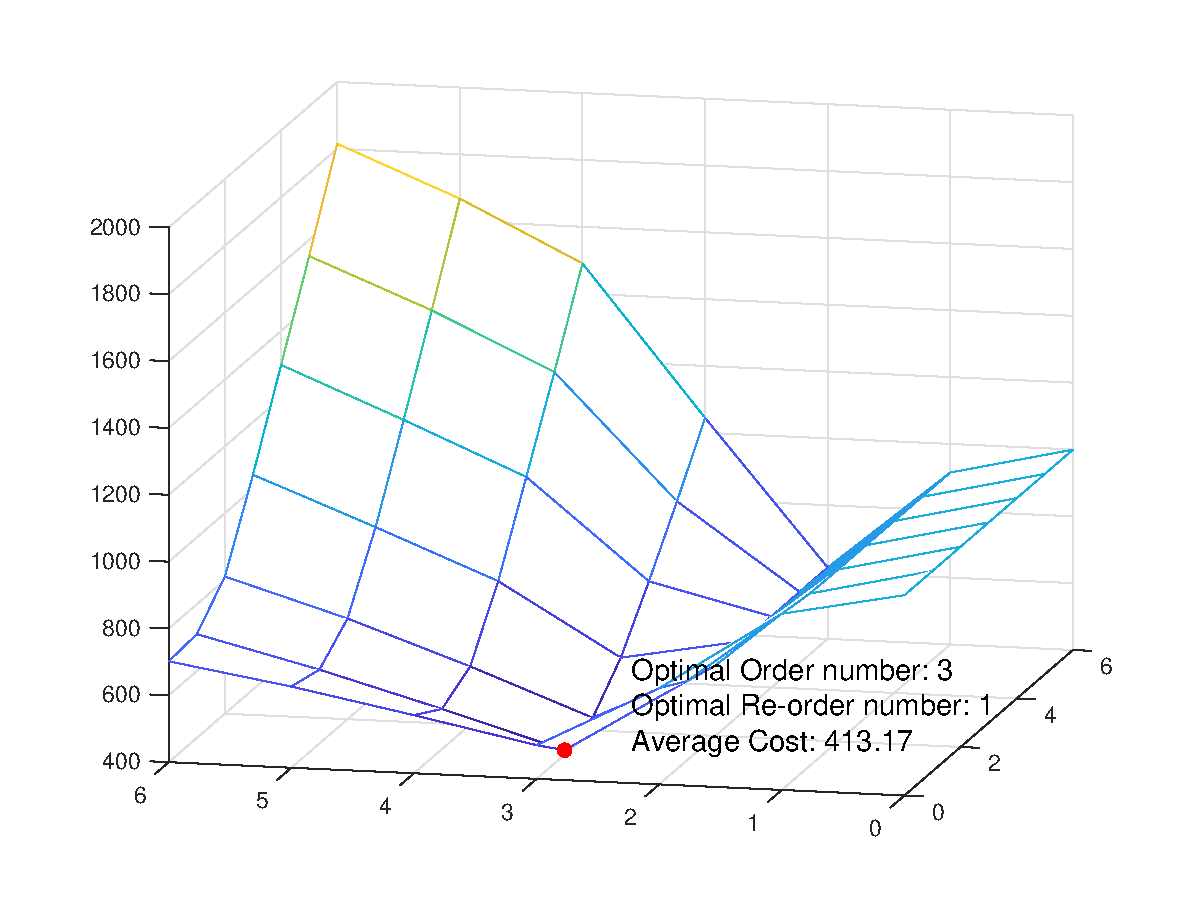
\includegraphics[width=0.4\textwidth]{t3.eps}
}}
   %\includegraphics[scale=1.0]{figurefile}
   \caption{Simulation result.}
\end{figure}


According to the simulation result, we get minimum cost at (3,1), which is exact what I choose without simulation. Some of the reason have been discussed previously.


The order number is mainly decided by the mean weekly cost of the distribution, which is 2.7 but we can only order integer number, then $y=3$. Under the same order number level, the advantage of $r=1$ is lower warehouse cost than $r=2$. On the contrary, the advantage of $r=2$ is that chance we be fined is low.


It is difficult to get a analytical solution of the expected respective cost. But since the weekly demand is mainly around 3 and $y=3$, then we can expected total penalty cost is lower than warehouse cost. Then $r=1$ achieves lower total cost.


In order to support such hypothesis, I change both penalty and warehouse cost in the simulation to see the optimal pair of (y,r) changes, which is shown in Table.2.


\begin{table}[h]
  \caption{Optimal (y,r) pair under different parameters}
  \label{table_example}
  \begin{center}
    \begin{tabular}{|c||c|c|c|c|c|c|c|}
      \hline
      Penalty   & 20 & 25 & 30 & 25 & 25 & 25 & 25\\
      \hline
      Warehouse & 5 & 5 & 5 & 3 & 4 & 6 & 10\\
      \hline
      y         & 3 & 3 & 3 & 3 & 3 & 3 & 3\\
      \hline
      r         & 1 & 1 or 2 & 2 & 2 & 2 & 1 & 1\\
      \hline
    \end{tabular}
  \end{center}
\end{table}
Under large penalty cost and low warehouse cost, $r=2$ tends to be better. On the opposite, when penalty cost is low and warehouse cost is high, $r=1$ tends to be best.


For task 4, we need to calculate the confidence interval of the total cost under specific cofidence $\alpha$ with respective (y,r) pair. According to the Central limit theorem(CLT), under large number of N, the total cost follows Gaussian distribution with mean an variance:
\begin{equation}
  \begin{split}
    & \mu =\lim\limits_{N \to \infty } \bar{X} = \lim\limits_{N \to \infty } \frac{1}{N}\sum_{i=1}^{N}X_i \\
    & \delta^2 =\lim\limits_{N \to \infty } S^2 = \lim\limits_{N \to \infty } \frac{1}{N-1}\sum_{i=1}^{N}(X_i-\bar{X})^2\\
  \end{split}
\end{equation}
Then, we can normalize each distribution with their mean and variance to a normal Gaussian distribution:
\begin{equation}
  \frac{X-\bar{X}}{S/\sqrt{N}} \sim  \mathtt{N}(0,1)
\end{equation}
Then we can use the cumulative distribution function(CDF) of normal Gaussian distribution ($z_\alpha$) to calculate the confidence interval. Here the confidence level(CL) $\alpha=99.999\%$. Then the confidence interval(CI) is:
\begin{equation}
  [L(X),U(X)] = [\bar{X}-z_{\alpha/2}\frac{\delta}{\sqrt{N}},\bar{X}+z_{\alpha/2}\frac{\delta}{\sqrt{N}}]
\end{equation}

According to Fig.3, (3,1) and (3,2)'s performance are extraordinary better than the others. Furthermore, since the Gaussian function drop exponentially, then the tail distribution of function with high mean value could be neglect. Then, here I only compare the confidence interval(CI) of (3,1) and (3,2), which result is shown below.
\begin{comment}
  \begin{table}[h]
    \caption{Confidence Interval under different confidence level}
    \label{table_example}
    \begin{center}
      \begin{tabular}{|c||c|c|c|c|c|c|c|}
        \hline
        \backslashbox{CI}{CL(\%)}   & 99 & 99.9 & 99.99 & 99.999\\
        \hline
        Lower bound (3,1)& 411.9 & 411.3 & 410.8 & 410.4 \\
        \hline
        Upper bound (3,1)& 415.9 & 416.5 & 417.0 & 417.4 \\
        \hline
        Lower bound (3,2)& 436.0 & 435.4 & 435.0 & 434.6 \\
        \hline
        Upper bound (3,2)& 439.9 & 440.5 & 441.0 & 441.4 \\
        \hline
      \end{tabular}
    \end{center}
  \end{table}
\end{comment}
\begin{figure}[thpb]
   \centering
   \framebox{\parbox{0.4\textwidth}{
   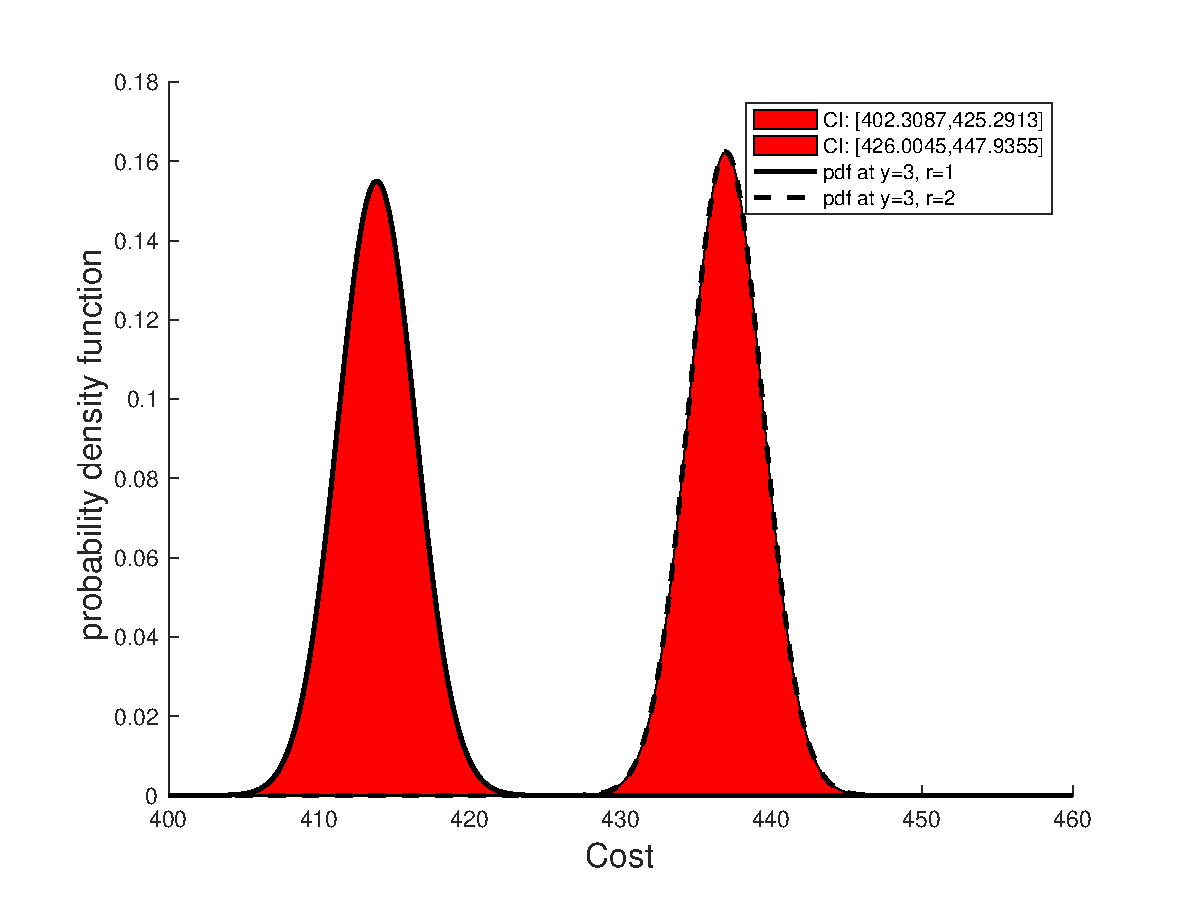
\includegraphics[width=0.4\textwidth]{t41.eps}
}}
   %\includegraphics[scale=1.0]{figurefile}
   \caption{Confidence interval for both pair at $\alpha =  99.999\%$}
\end{figure}


According to Fig.4, the upper bound of (3,1) is still less than the lower bound of (3,2), which means we have at least $0.99999^2$ confidence that the cost for (3,1) and (3,2) are inside their confidence interval respectively and then cost for (3,1) is less than (3,2), which is strong enough.

In order to improve the confidence, we can increase the simulation run length (e.g N = 5000), which will narrow the confidence interval under same confidence level ($z_\alpha$ remain the same). According to CLT, sample variance $S^2$ equals to distribution variance $\delta^2$, which is fixed and then:
\begin{equation}
  \lim\limits_{N \to \infty } z_\alpha \frac{\delta}{\sqrt{N}} = 0
\end{equation}
Then the confidence interval $[\bar{X}-z_{\alpha/2}\frac{\delta}{\sqrt{N}},\bar{X}+z_{\alpha/2}\frac{\delta}{\sqrt{N}}]$ will be narrowed under same $\alpha$.
\section{Conclusion (Task \uppercase\expandafter{\romannumeral5})}
 Since the high confidence, I suppose the the objectives is achieved. During the simulation, I found increase run length can extremely narrow the confidence interval of our results, but it will also takes much more time to process the simulation. Besides, the time is heavily used to generate random numbers, which indicate the MATLAB built in function \textsl{unidrnd(.)} and rejection method have low efficiency.


 Under the scenario of solving practical problem, it is of vital importance to find an effective way to generate random numbers as well as an appropriate run length N. Finally, it is also important to find a way to evaluate results.



\addtolength{\textheight}{-12cm}
 % This command serves to balance the column lengths
% on the last page of the document manually. It shortens
                                  % the textheight of the last page by a suitable amount.
                                  % This command does not take effect until the next page
                                  % so it should come on the page before the last. Make
                                  % sure that you do not shorten the textheight too much.


\end{document}
